\documentclass{beamer}

% --- THEME AND STYLING ---
\usetheme{default}
\usecolortheme{default}

% --- PACKAGES ---
\usepackage[utf8]{inputenc}
\usepackage{amsmath, amssymb, amsfonts}
\usepackage{graphicx}
\usepackage{booktabs} % For professional-looking tables
\usepackage{xcolor}   % For colored boxes
\usepackage{fontawesome5} % For icons if needed
\usepackage{hyperref}

% --- PRESENTATION METADATA ---
\title{Learning Patient-Specific Lung Deformation from 4D-CT}
\author{Your Name / Your Group}
\institute{Your Institution}
\date{\today}

\begin{document}

% --- TITLE PAGE ---
\begin{frame}
  \titlepage
\end{frame}

% --- TABLE OF CONTENTS ---
\begin{frame}{Outline}
  \tableofcontents
\end{frame}

% ===================================================================
\section{Overview}
% ===================================================================

\begin{frame}[fragile]{Introduction \& Motivation}
Goal

        This presentation summarizes the data, notation, and end-to-end pipeline used to simulate and learn patient-specific lung deformation from 4D-CT.
    
        We denote the displacement field computed by non-rigid image registration as:
        \[
          \mathbf{u}_{\mathrm{true}} \colon \Omega \subset \mathbb{R}^3 \to \mathbb{R}^3
        \]
        This field is calculated between a \emph{reference} phase (e.g., end-exhalation, EE) and a \emph{target} phase (e.g., end-inspiration, EI).
        \newline\vspace{0.5cm}
        At each location $\mathbf{x}\in\Omega$, the vector $\mathbf{u}_{\mathrm{true}}(\mathbf{x})$ specifies how the reference image must move to align with the target.
    
\end{frame}

% ---
\subsection{Data and Pipeline}
% ---

\begin{frame}[fragile]{Data Specification}
    \frametitle{Data Entities Used by the Pipeline}
    The primary entities manipulated by our framework are listed below. The volumetric mesh is generated only once and reused for all phases.
    \vspace{1em}
    \begin{beamercolorbox}[sep=0.5em]{block body}
    \tiny
    \begin{tabular}{@{}lp{8cm}@{}}
    \toprule
    \textbf{Symbol / File} & \textbf{Description} \\
    \midrule
    $I_i\colon \Omega \to \mathbb{R}$ & 3D CT volume at respiratory phase $i$ (0\%, 10\%, \dots, 90\%), where 0\% is EE and 50\% is EI. \\[1.5em]
    Segmentation mask & Multi-class volume identifying lung parenchyma, airways, etc. Used to define the computational domain and extract the surface $\partial\Omega$. \\[1.5em]
    Volumetric mesh $\mathcal{T}=(\mathbf{V},\mathbf{E},\mathbf{T})$ & Generated once from the segmentation mask; provides vertices, edges, and tetrahedra for the mass–spring system. \\[1.5em]
    Ground-truth displacement $\mathbf{u}_{\mathrm{true}}$ & Dense vector field from registration (Eq.~\eqref{eq:registration}). Interpolated on $\partial\Omega$ to prescribe Dirichlet conditions. \\[1.5em]
    Material labels $c(v)$ or intensities $I(v)$ & Node-/element-wise features for the neural network that predicts stiffness. \\
    \bottomrule
    \end{tabular}
    \end{beamercolorbox}
\end{frame}

\begin{frame}{Data Flow: Segmentation to Boundary Conditions}
    \begin{exampleblock}{Segmentation vs. Boundary Conditions}
    A segmentation mask encodes \emph{shape only}. The registration field provides the \emph{motion data}.
    \end{exampleblock}
    
    The flow is as follows:
    \begin{enumerate}
      \item \emph{Segmentation} $\longrightarrow$ domain $\Omega$ and boundary mesh;
      \item \emph{Registration} $\longrightarrow$ displacement vectors on $\Omega$;
      \item Sampling $\mathbf{u}_{\mathrm{true}}$ on $\partial\Omega$ $\longrightarrow$ prescribed displacements $\mathbf{u}_i$.
    \end{enumerate}
    The simulator never consumes the mask directly as a boundary condition.
\end{frame}

\begin{frame}[fragile]{Image Registration Formulation}
    \frametitle{Ground Truth Estimation via Image Registration}
    For a given pair $(I_{\mathrm{ref}}, I_{\mathrm{tar}})$, we estimate $\mathbf{u}_{\mathrm{true}}$ by solving the following optimization problem:
    \begin{equation}
    \label{eq:registration}
    \min_{\mathbf{u}}
      \int_{\Omega} \bigl|I_{\mathrm{tar}}(\mathbf{x}) - I_{\mathrm{ref}}(\mathbf{x} + \mathbf{u}(\mathbf{x}))\bigr|^2 \,\mathrm{d}\mathbf{x}
      + \lambda \int_{\Omega} \lVert\nabla \mathbf{u}(\mathbf{x})\rVert^2 \,\mathrm{d}\mathbf{x},
    \end{equation}
    with the regularization parameter $\lambda\in[10^{-2},10^{-1}]$.
    \vfill
    \begin{alertblock}{}
    This computationally expensive step is pre-processed and the resulting $\mathbf{u}_{\mathrm{true}}$ fields are stored as data.
    \end{alertblock}
\end{frame}

\begin{frame}[fragile]{End-to-End Processing Pipeline}
    \frametitle{Summary of Processing Steps}
    \begin{beamercolorbox}[sep=0.5em]{block body}
    \tiny
    \begin{tabular}{@{}p{1.2cm}p{3.5cm}p{5.5cm}@{}}
    \toprule
    \textbf{Step} & \textbf{Input \(\to\) Output} & \textbf{Key operation} \\
    \midrule
    1 & \((I_{\mathrm{ref}},I_{\mathrm{tar}})\to\mathbf{u}_{\mathrm{true}}\) &
      Solve registration problem; saved as files. \\[1em]
    2 & Mask \(\to \mathcal{T}\) &
      Generate tetrahedral mesh (cached). \\[1em]
    3 & \(k \to \mathbf{u}_{\mathrm{sim}} = g(k)\) &
      Forward spring–mass solve: enforce \(\nabla_{\mathbf{q}}U(k,\mathbf{q}) = \mathbf{0}\), then compute \(\mathbf{u}_{\mathrm{sim}} = \mathbf{q} - \mathbf{X}.\) \\[1em]
    4 & \(\mathbf{u}_{\mathrm{true}}\to k^*\) & 
      Inverse problem:
      \(\displaystyle
        k^* = \arg\min_k \Bigl\lVert \mathbf{u}_{\mathrm{true}}
        - \mathbf{u}_{\mathrm{sim}}(k)\Bigr\rVert^2
        + \gamma\,\|\nabla k\|^2
      \)\\[2em]
    5 & \((I_i, k^*)\to \theta^*\) &
      Learning: train ANN \(k_\theta = f_\theta(I)\) via
      \(\displaystyle
        \theta^* = \arg\min_\theta 
        \mathbb{E}_{\mathrm{cases}}
        \Bigl\lVert \mathbf{u}_{\mathrm{true}}
        - \mathbf{u}_{\mathrm{sim}}\bigl(f_\theta(I)\bigr)\Bigr\rVert^2.
      \) \\
    \bottomrule
    \end{tabular}
    \end{beamercolorbox}
\end{frame}

\begin{frame}[fragile]{Three Levels of the Problem}
\small
    \begin{block}{Level 1 (Forward Problem)}
    Given a stiffness field \(k(\mathbf{x})\), solve for the simulated displacement:
    \[
      g(k):\quad
      \frac{\partial U(k,\mathbf{q})}{\partial \mathbf{q}} = \mathbf{0},
      \qquad
      \mathbf{u}_{\mathrm{sim}} = \mathbf{q} - \mathbf{X}.
    \]
    Where $U(k,\mathbf{q})$ is the total potential energy, $\mathbf{q}$ are deformed coordinates, and $\mathbf{X}$ are reference coordinates.
    \end{block}
    
    \begin{block}{Level 2 (Inverse Problem)}
    Directly optimize the stiffness field:
    \[
      k^* = \arg\min_k
         \bigl\lVert \mathbf{u}_{\mathrm{true}}
         - \mathbf{u}_{\mathrm{sim}}(k)\bigr\rVert^2
    ,
    \]
    \end{block}
    \begin{block}{Level 3 (Learning)}
    Learn a mapping $f_\theta$ from image to stiffness:
    \[
      \theta^* = \arg\min_\theta
         \mathbb{E}_{\mathrm{cases}}
         \bigl\lVert \mathbf{u}_{\mathrm{true}}
         - \mathbf{u}_{\mathrm{sim}}\bigl(f_\theta(I)\bigr)\bigr\rVert^2.
    \]
    \end{block}
\end{frame}



% ===================================================================
\section{Spring Mass System Approach}
% ===================================================================
\subsection{System Definition}

\begin{frame}[fragile]{Introduction to Mass-Spring Systems (MSM)}
    \begin{block}{Forward Simulation Model}
    We model the deformable tissue (e.g., lung) as a Mass-Spring System (MSM). This system consists of a grid of particles (mass points) interconnected by a network of springs, which approximates the continuous mechanics of the tissue.
    \end{block}
    
    \begin{columns}
        \begin{column}{0.5\textwidth}
            \textbf{System State}
            \begin{itemize}
                \item \textbf{Mass} $m_i$: Assumed identical for all particles.
                \item \textbf{Position} $\mathbf{x}_i(t) \in \mathbb{R}^3$.
                \item \textbf{Velocity} $\mathbf{v}_i(t) = \dot{\mathbf{x}}_i(t)$.
            \end{itemize}
            \vspace{1em}
            \textbf{Dynamics} (Newton's 2nd Law):
            \begin{equation*}
                m_i \ddot{\mathbf{x}}_i(t) = \mathbf{F}_i(\mathbf{x}, \dot{\mathbf{x}})
            \end{equation*}
        \end{column}
        \begin{column}{0.5\textwidth}
            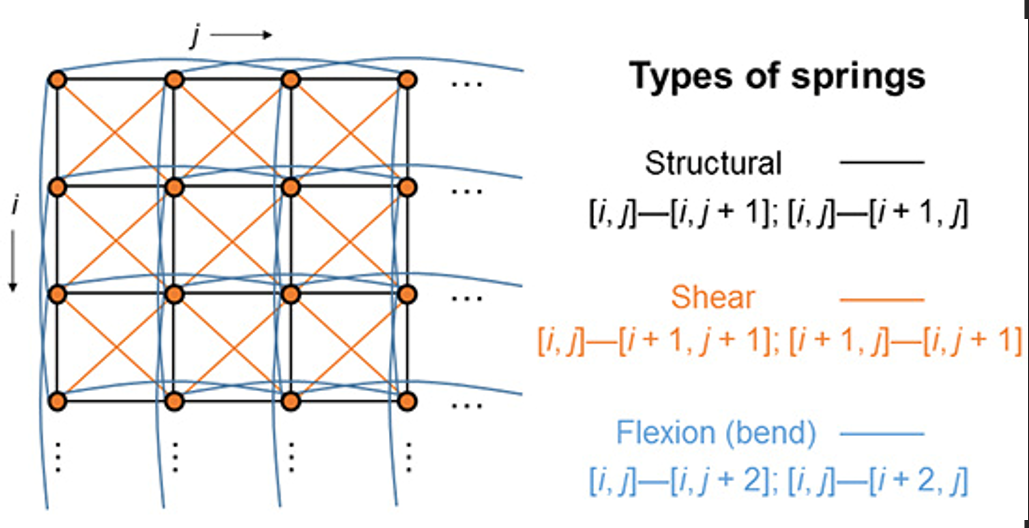
\includegraphics[width=\textwidth]{images/fig2.0.png}
        \end{column}
    \end{columns}
\end{frame}

\begin{frame}[fragile]{Spring Forces and Types}
    \textbf{Spring Forces (Hooke's Law)}
    For a spring connecting particles at $\mathbf{p}$ and $\mathbf{q}$ with stiffness $k$ and rest length $L_0$, the force on $\mathbf{p}$ is:
    \begin{equation} \label{eq:spring_force_slide}
        \mathbf{F}_{\text{spring}} = k (L_0 - \lVert \mathbf{p} - \mathbf{q} \rVert) \frac{\mathbf{p} - \mathbf{q}}{\lVert \mathbf{p} - \mathbf{q} \rVert}
    \end{equation}
    
    \textbf{Spring Types for Stability}
    \begin{itemize}
        \item \textbf{Structural springs:} Connect adjacent particles to resist stretching.
        \item \textbf{Shear springs:} Connect diagonal neighbors to resist shearing.
        \item \textbf{Flexion (bend) springs:} Connect particles two steps away to resist bending.
    \end{itemize}
    
    \textbf{Time Integration (Explicit Euler)}
    \[
      \mathbf{v}_i(t+\Delta t)
        = \mathbf{v}_i(t)
        + \Delta t\;\frac{\mathbf{F}_i\bigl(\mathbf{x}(t),\mathbf{v}(t)\bigr)}{m}
    \]
    \[
      \mathbf{x}_i(t+\Delta t)
        = \mathbf{x}_i(t)
        + \Delta t\;\mathbf{v}_i(t).
    \]
\end{frame}
%===================================================================
% NEW SLIDE: Implicit Dynamic Solver Derivation
%===================================================================

% --- SLIDE 1: GOAL AND UPDATE RULES ---
\begin{frame}[fragile]
    \frametitle{Dynamic Solver: Implicit Euler Method}

    \begin{alertblock}{Goal}
        To solve the dynamic equation of motion $\mathbf{M}\ddot{\mathbf{q}} = \mathbf{F}(\mathbf{q})$ over a time step $\Delta t$. Unlike Explicit Euler, this method is unconditionally stable, making it ideal for stiff systems like springs.
    \end{alertblock}

    \begin{block}{1. Implicit Euler Update Rules}
        The velocity and position are updated using the state at the \textbf{end} of the time step ($n+1$):
        \begin{align*}
            \mathbf{v}^{n+1} &= \mathbf{v}^n + \Delta t \cdot \mathbf{a}^{n+1} \\
            \mathbf{q}^{n+1} &= \mathbf{q}^n + \Delta t \cdot \mathbf{v}^{n+1}
        \end{align*}
        The system's governing equation is $\mathbf{M}\mathbf{a}^{n+1} = \mathbf{F}(\mathbf{q}^{n+1})$.
    \end{block}
\end{frame}

% --- SLIDE 2: DERIVATION (PART 1) ---
\begin{frame}[fragile]
\small
    \frametitle{Implicit Euler Derivation (Part 1)}
    
        Our goal is to find the position update $\Delta\mathbf{q} = \mathbf{q}^{n+1} - \mathbf{q}^n$.
        \begin{enumerate}
            \item the last equation could be in terms of velocity:
            \[
                \mathbf{M}\frac{\mathbf{v}^{n+1} - \mathbf{v}^n}{\Delta t} = \mathbf{F}(\mathbf{q}^{n+1})
            \]
            \item Next, express the unknown velocity $\mathbf{v}^{n+1}$ in terms of the position update $\Delta\mathbf{q}$:
            \[
                \mathbf{v}^{n+1} = \frac{\mathbf{q}^{n+1} - \mathbf{q}^n}{\Delta t} = \frac{\Delta\mathbf{q}}{\Delta t}
            \]
            \item Substitute this into the equation from step 1:
            \[
                \mathbf{M}\frac{(\Delta\mathbf{q}/\Delta t) - \mathbf{v}^n}{\Delta t} = \mathbf{F}(\mathbf{q}^{n+1}) \implies \mathbf{M}(\Delta\mathbf{q} - \Delta t\,\mathbf{v}^n) = (\Delta t)^2 \mathbf{F}(\mathbf{q}^{n+1})
            \]
            \item The force $\mathbf{F}(\mathbf{q}^{n+1})$ depends on the unknown future state. We linearize it around the current state $\mathbf{q}^n$:
            \[
                \mathbf{F}(\mathbf{q}^{n+1}) = \mathbf{F}(\mathbf{q}^n + \Delta\mathbf{q}) \approx \mathbf{F}(\mathbf{q}^n) + \frac{\partial \mathbf{F}}{\partial\mathbf{q}}\bigg|_{\mathbf{q}^n} \Delta\mathbf{q} = \mathbf{F}(\mathbf{q}^n) - \mathbf{K}_T \Delta\mathbf{q}
            \]
        \end{enumerate}
    
\end{frame}

% --- SLIDE 3: DERIVATION (PART 2) ---
\begin{frame}[fragile]
    \frametitle{Implicit Euler Derivation (Part 2)}
    \begin{block}{2. Detailed Derivation (continued)}
        \begin{enumerate}
            % This command continues the numbering from the previous slide.
            % 这个命令让列表编号从上一页继续。
            \setcounter{enumi}{4} 
            
            \item Substitute the linearized force back and group terms with the unknown $\Delta\mathbf{q}$ on the left:
            \[
                \mathbf{M}(\Delta\mathbf{q} - \Delta t\,\mathbf{v}^n) \approx (\Delta t)^2 (\mathbf{F}(\mathbf{q}^n) - \mathbf{K}_T \Delta\mathbf{q})
            \]
            Which simplifies to:
            \[
                \mathbf{M}\Delta\mathbf{q} + (\Delta t)^2 \mathbf{K}_T \Delta\mathbf{q} \approx (\Delta t)^2 \mathbf{F}(\mathbf{q}^n) + \Delta t\,\mathbf{M}\mathbf{v}^n
            \]
        \end{enumerate}
    \end{block}
\end{frame}

% --- SLIDE 4: FINAL SYSTEM ---
\begin{frame}[fragile]
    \frametitle{Implicit Euler: The Final Ax=b System}
    \begin{exampleblock}{3. The Final \texttt{Ax=b} System}
        Factoring out $\Delta\mathbf{q}$ from the previous step gives the final linear system:
        \[
            \underbrace{\left( \mathbf{M} + (\Delta t)^2 \mathbf{K}_T \right)}_{\mathbf{A}} \underbrace{\Delta\mathbf{q}}_{\mathbf{x}} = \underbrace{\Delta t \left( \mathbf{M}\mathbf{v}^n + \Delta t\,\mathbf{F}(\mathbf{q}^n) \right)}_{\mathbf{b}}
        \]
        At each time step, we solve this system for $\Delta\mathbf{q}$ and update the position: $\mathbf{q}^{n+1} = \mathbf{q}^n + \Delta\mathbf{q}$.
    \end{exampleblock}
\end{frame}
% ---
\subsection{Topology for Volumetric Mesh}
% ---

\begin{frame}[fragile]{Volumetric Topology: Intersection Points}
    \begin{block}{Concept}
    In each tetrahedral element $\mathcal V_k$, we define a local coordinate system by finding six intersection points $q_{j}$. These are found by ray-casting from the barycenter $x_b$ along three anisotropy axes to the faces.
    \end{block}
    
    \textbf{Barycenter Calculation}
    \[
        x_b \;=\;\frac{1}{4}\sum_{i=1}^4 x_i
    \]
    
    \textbf{Point-in-triangle Test}
    
    A point $q_j$ is on a face $\Delta_{i_1i_2i_3}$ if the sum of sub-triangle areas equals the total area:
    \[
        S_{\Delta_{i_1i_2i_3}} \;=\; S_{\Delta_{q_j\,i_2\,i_3}} + S_{\Delta_{i_1\,q_j\,i_3}} + S_{\Delta_{i_1\,i_2\,q_j}}.
    \]
\end{frame}

\begin{frame}[fragile]{Volumetric Topology: Coefficient Matrix}
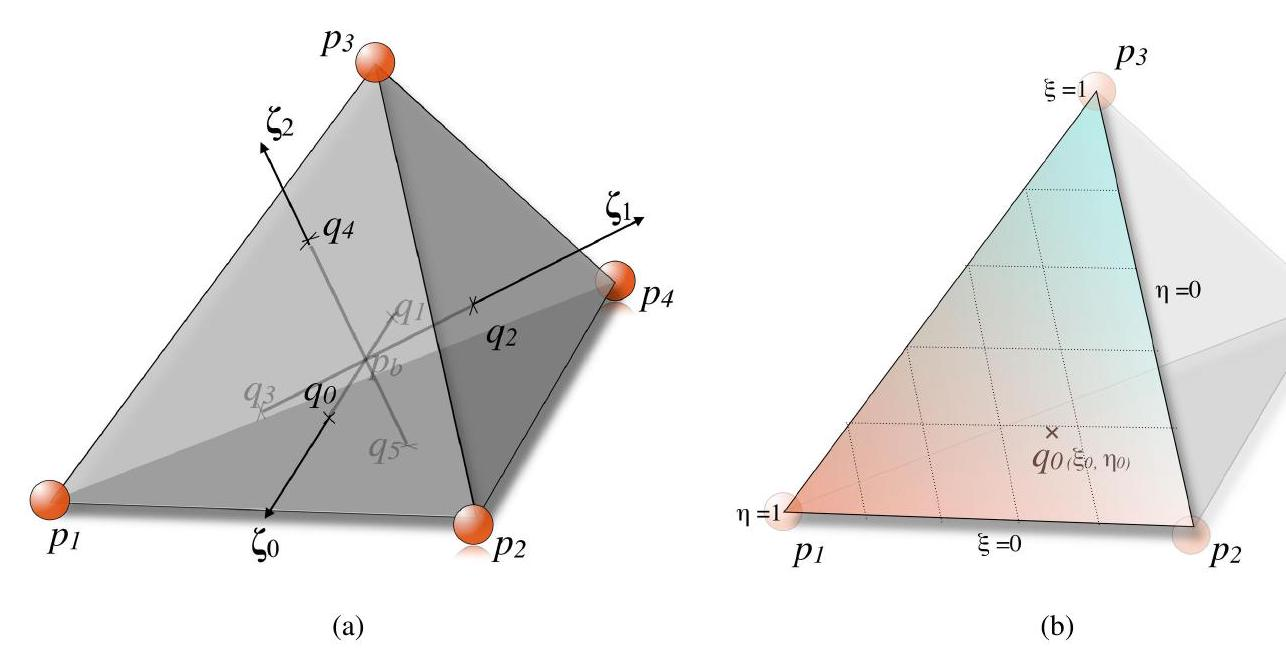
\includegraphics[width=\textwidth]{images/fig2.6.jpg}
\end{frame}

\begin{frame}[fragile]{Volumetric Topology: Coefficient Matrix}

            \textbf{Barycentric Coordinates}
            
            The local coordinates of $q_j$ on a face are ratios of areas:
            \begin{align*}
                \xi &= \frac{S_{\Delta_{q_j\,i_2\,i_3}}}{S_{\Delta_{i_1i_2i_3}}} \\
                \eta &= \frac{S_{\Delta_{q_j\,i_1\,i_3}}}{S_{\Delta_{i_1i_2i_3}}}
            \end{align*}
            
            \textbf{Coefficient Matrix $C^k$}
            
            We build a $4 \times 6$ matrix $C^k$ where each entry is the value of a shape function $N_i$ at an intersection point $q_j$:
            \[
                C^k_{ij}\;=\;N_i\bigl(q_j\bigr)
            \]

    
    \textbf{Updating Intersections}
    At runtime, intersection points move with the vertices:
    \[
        x^t_j \;=\;\sum_{i=1}^4 C^k_{ij}\;x^t_i
    \]
\end{frame}

% ---
\subsection{Internal Forces}
% ---

\begin{frame}{Internal Forces: Axial and Torsion Springs}
    \begin{block}{Force Calculation Strategy}
    Internal forces in each tetrahedron are computed by:
    \begin{itemize}
        \item \textbf{Three axial springs} along the anisotropy axes.
        \item \textbf{Three torsion springs} coupling each pair of axes.
    \end{itemize}
    \end{block}
    \begin{center}
        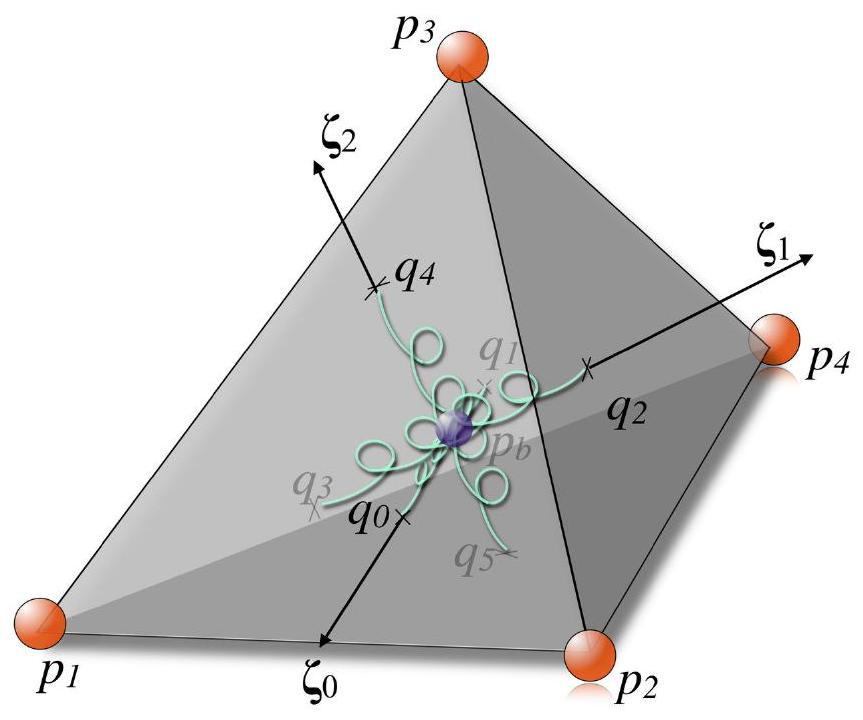
\includegraphics[width=0.4\textwidth]{images/fig2.12.jpg}
    \end{center}
\end{frame}

\begin{frame}[fragile]{Internal Forces: Axial Springs}
    \begin{itemize}
        \item \textbf{Axis vectors}: Along axis $\ell$, the vector between two intersection points is:
        \[
        \zeta_\ell^t = x^t_{q_{\ell,1}} - x^t_{q_{\ell,2}}.
        \]
        
        \item \textbf{Initial length} (at $t=0$):
        \[
        l^0_\ell = \|\zeta_\ell^0\| = \bigl\|\,x^0_{q_{\ell,1}}-x^0_{q_{\ell,2}}\,\bigr\|.
        \]
        
        \item \textbf{Unit direction}:
        \[
        \hat\zeta_\ell^t = \frac{\zeta_\ell^t}{\|\zeta_\ell^t\|}.
        \]
        
        \item \textbf{Hooke’s law} (linear axial force):
        \begin{equation*}
        \boxed{
        f^{t}_{\ell,\,\mathrm{axial}} = -\,k_\ell\bigl(\|\zeta_\ell^t\| - \|\zeta_\ell^0\|\bigr)\,\hat\zeta_\ell^t
        }
        \end{equation*}
        where $k_\ell$ is the stiffness constant.
    \end{itemize}
\end{frame}

\begin{frame}[fragile]{Internal Forces: Torsion Springs}
    \begin{block}{Concept}
    Torsion springs penalize deviations of the angles between anisotropy axes from their rest values.
    \end{block}
    
    \textbf{1. Angle between two axes ($\ell, m$)}
    \[
        \alpha^t_{\ell m} = \arccos\bigl(\hat\zeta_\ell^t \!\cdot\! \hat\zeta_m^t\bigr), \quad \alpha^0_{\ell m} = \text{rest angle}
    \]
    
    \textbf{2. Torsion Force Derivation}
    
    The force is derived from a potential energy $U_\tau = \tfrac12\sum_{p\in\{m,n\}} k_{\ell p}\,\bigl(\alpha^t_{\ell p}-\alpha^0_{\ell p}\bigr)^2$. This gives the force magnitude:
    \[
        f_\tau(\zeta_\ell,\alpha_{\ell m},\alpha_{\ell n}) = -\,k_{\ell m}\,\bigl(\alpha^t_{\ell m}-\alpha^0_{\ell m}\bigr)
    \]
\end{frame}

\begin{frame}[fragile]{Torsion Spring Models}
    \textbf{3. Linear Torsion-Spring Model}
    The force generated by the spring between axes $\ell$ and $m$, acting on axis $\ell$, is directed along axis $m$:
    \begin{equation*}
    \boxed{
    f^t_{\ell\to m} = -\,k_{\ell m}\,\bigl(\alpha^t_{\ell m}-\alpha^0_{\ell m}\bigr)\,\hat\zeta_m^t
    }
    \end{equation*}
    
    \textbf{4. Cosine-Approximation (for small angles)}
    When axes remain nearly orthogonal, the angle difference can be approximated by the difference in dot products:
    \begin{equation*}
    \boxed{
    f^t_{\ell\to m} = -\,k_{\ell m}\,\bigl((\hat\zeta_\ell^t\!\cdot\!\hat\zeta_m^t) - (\hat\zeta_\ell^0\!\cdot\!\hat\zeta_m^0)\bigr)\,\hat\zeta_m^t
    }
    \end{equation*}
    
    \begin{alertblock}{Assembly}
    Each tetrahedron contributes 6 axial-spring forces and 6 torsion-spring forces, which are distributed to the four vertices via the coefficient matrix $C^k$.
    \end{alertblock}
\end{frame}

% ---
\subsection{Volume Preservation}
% ---

\begin{frame}[fragile]{Simplified Volume Preservation}
    \begin{block}{Barycentric Volume Springs}
    To control tetrahedral volume, we connect each vertex to the element's barycenter.
    \end{block}
    \begin{enumerate}
        \item \textbf{Current barycenter}: $x_b^t=\frac{1}{4}\sum_{i=1}^4 x_i^t$.
        \item \textbf{Radial vectors}: $\xi^t_j=x_b^t - x_j^t$.
        \item \textbf{Rest lengths} $\|\xi^0_j\|$ are computed at $t=0$.
        \item \textbf{Total length error}: $\Delta L=\sum_{j=1}^4\|\xi_j^t\| \;-\;\sum_{j=1}^4\|\xi_j^0\|$.
        \item \textbf{Barycentric spring force} on node $j$:
        \[
            f^t_j = -\,k_s\,\Delta L\,\frac{\xi^t_j}{\|\xi^t_j\|} \;-\;c\,(v_j^t - v_b^t)
        \]
        \item \textbf{Adaptive stiffness update}:
        \[
            k_s^{t+\Delta t} = k_s^t + \mu\,\Delta V\,\sum_{j=1}^4\|\xi_j^t\|,
        \]
        where $\Delta V=V^t-V^0$ is the volume error.
    \end{enumerate}
\end{frame}


% ===================================================================
\section{Static Equilibrium Solver}
% ===================================================================
\subsection{Boundary Conditions}

\begin{frame}[fragile]{Static Solver: Boundary Conditions}
    \begin{block}{Dirichlet Boundary $\Gamma_D$}
    Nodes on this boundary have their positions explicitly prescribed.
    \[
        \mathbf{q}_D = \mathbf{X}_D + \mathbf{u}_i
    \]
    Where $\mathbf{u}_i$ is the ground-truth displacement from image registration.
    \end{block}
    
    \begin{block}{Neumann Boundary $\Gamma_N$}
    Nodes on this boundary are subjected to external forces (e.g., pressure). The equivalent nodal force is:
    \[
        [\mathbf{F}_{\text{ext}}]_i = \int_{\Gamma_N} N_i(\mathbf{s})\,\mathbf{t}(\mathbf{s})\,\mathrm{d}S
    \]
    Where $\mathbf{t}(\mathbf{s})$ is the surface traction and $N_i(\mathbf{s})$ is the FE shape function.
    \end{block}
\end{frame}

\begin{frame}[fragile]{Static Solver: System Partitioning}
    We partition the global coordinate and external force vectors into free (F) and constrained/Dirichlet (D) components:
    \[
      \mathbf{F}_{\text{ext}} = 
      \begin{bmatrix}
          \mathbf{F}_{F,\text{ext}}\\[4pt]
          \mathbf{F}_{D,\text{ext}}
      \end{bmatrix},
      \quad
      \mathbf{q} = 
      \begin{bmatrix}
          \mathbf{q}_F\\[2pt]
          \mathbf{q}_D
      \end{bmatrix},
    \]
    \begin{itemize}
        \item $\mathbf{q}_F$: The unknown coordinates of the free nodes.
        \item $\mathbf{F}_{F,\text{ext}}$: External forces on the free nodes.
        \item $\mathbf{F}_{D,\text{ext}}$: External forces on fixed nodes (used for reaction force analysis).
    \end{itemize}
\end{frame}

% ---
\subsection{Newton-Raphson Method}
% ---

\begin{frame}[fragile]{Static Solver: Energy and Residual}
    \textbf{Internal Potential Energy}
    The total energy stored in all springs is:
    \[
      U(k,\mathbf{q}) = \sum_{e\in\mathcal{T}}\;\sum_{(i,j)\in e} \frac{1}{2}\,k_{ij}\,\|\mathbf{q}_i - \mathbf{q}_j\|^2.
    \]
    
    \textbf{Internal Force Vector}
    The internal force is the gradient of the potential energy:
    \[
      \mathbf{g}_{\text{int}}(\mathbf{q}) = \nabla_{\mathbf{q}} \,U(k,\mathbf{q})
    \]
    
    \textbf{Equilibrium Residual}
    Static equilibrium is reached when internal forces balance external forces. The residual vector is:
    \[
      \mathbf{r}(\mathbf{q}) = \mathbf{g}_{\text{int}}(\mathbf{q}) + \mathbf{F}_{\text{ext}}
    \]
    We need to solve for $\mathbf{q}$ such that the residual on the free nodes is zero: $\mathbf{r}_F = \mathbf{g}_F + \mathbf{F}_{F,\text{ext}} = \mathbf{0}$.
\end{frame}

\begin{frame}[fragile]{Newton-Raphson Iteration}
    We solve the non-linear system $\mathbf{r}(\mathbf{q}) = \mathbf{0}$ iteratively.
    
    \textbf{Stiffness Matrix}
    The stiffness matrix is the Hessian of the internal potential energy:
    \[
      \mathbf{K}_T(\mathbf{q}) = \frac{\partial^2 U}{\partial \mathbf{q}^2} = \frac{\partial \mathbf{g}_{\text{int}}}{\partial \mathbf{q}}
    \]
    
    \textbf{Linearized Residual}
    At the current iterate $\mathbf{q}^{(k)}$, we use a Taylor expansion:
    \[
      \mathbf{r}(\mathbf{q}^{(k)} + \Delta\mathbf{q})
      \approx
        \mathbf{r}(\mathbf{q}^{(k)})
      + \mathbf{K}_T^{(k)} \Delta\mathbf{q}.
    \]
    
    \textbf{Incremental Equation}
    Setting the linearized residual to zero gives a linear system for the update $\Delta\mathbf{q}$:
    \[
      \mathbf{K}_T^{(k)}\,\Delta\mathbf{q} = -\,\mathbf{r}(\mathbf{q}^{(k)}) = -\bigl[\mathbf{g}_{\text{int}}(\mathbf{q}^{(k)}) + \mathbf{F}_{\text{ext}}\bigr].
    \]
\end{frame}

\begin{frame}[fragile]{Newton-Raphson: Handling BCs}
    \textbf{Partitioning the System}
    We partition the stiffness matrix $\mathbf{K}_T$ and residual $\mathbf{r}$:
    \[ K_T=\begin{bmatrix}K_{F F} & K_{F D} \\ K_{D F} & K_{D D}\end{bmatrix}, \quad \mathbf{r}=\begin{bmatrix}\mathbf{r}_F \\ \mathbf{r}_D\end{bmatrix} \]
    
    \textbf{The Free-DOF Subsystem}
    By substituting $\Delta\mathbf{q}=[\Delta\mathbf{q}_F;\mathbf{0}]$ into the incremental equation, we arrive at the reduced system for the free degrees of freedom:
    \[
      \mathbf{K}_{FF}^{(k)}\,\Delta\mathbf{q}_F = -\,\mathbf{r}_F(\mathbf{q}^{(k)}) = -\bigl[\mathbf{g}_F(\mathbf{q}^{(k)}) + \mathbf{F}_{F,\text{ext}}\bigr].
    \]
    
    \textbf{Update and Convergence}
    The update step is:
    \[
        \mathbf{q}_F^{(k+1)} = \mathbf{q}_F^{(k)} + \Delta\mathbf{q}_F, \quad \mathbf{q}_D^{(k+1)} = \mathbf{q}_D.
    \]
    We iterate until $\lVert\mathbf{r}_F(\mathbf{q}^{(k+1)})\rVert$ is below a threshold.
\end{frame}

\begin{frame}[fragile]{Special Case: All-Dirichlet Systems}
    \begin{alertblock}{What happens to external forces on Dirichlet nodes?}
    They do not affect the free nodes' solution; instead, they become part of the reaction forces.
    \end{alertblock}
    
    This can be shown with an augmented potential function using Lagrange multipliers $\boldsymbol\lambda$ (the reaction forces):
    \[
        \Pi(\mathbf{q},\boldsymbol\lambda) = U(k, \mathbf{q}) + \mathbf{F}_{\text{ext}}^{\!\top}\mathbf{q} + \boldsymbol\lambda^{\!\top} \bigl(\mathbf{q}_D - \mathbf{X}_D - \mathbf{u}_i\bigr).
    \]
    
    If $\mathbf{F}_{F,\text{ext}} = \mathbf{0}$ (no external forces on free nodes), solving the saddle-point system shows that the linear system for free DOFs degenerates to:
    \[
        \boxed{ \mathbf{K}_{FF}\,\Delta\mathbf{q}_F = -\,\mathbf{g}_F }
    \]
    The external forces $\mathbf{F}_{D,\text{ext}}$ are entirely balanced by the reaction forces $\boldsymbol{\lambda}$.
\end{frame}

\begin{frame}[fragile]{Static Solver: Final Output}
    \begin{itemize}
        \item \textbf{Linear Subproblem}: In the general case, we solve this at each iteration, often with the Conjugate Gradient method:
        \[
            \mathbf{K}_{FF}\,\Delta\mathbf{q}_F = -\bigl[\mathbf{g}_F + \mathbf{F}_{F,\text{ext}}\bigr]
        \]
    
        \item \textbf{Simulated Displacement}: After convergence, the final displacement field is:
        \[
           \mathbf{u}_{\text{sim}} = \mathbf{q} - \mathbf{X}.
        \]
    
        \item \textbf{Reaction Forces (Optional)}: The forces at the Dirichlet boundary can be calculated for analysis:
        \[
           \boldsymbol{\lambda} = -(\mathbf{g}_D(\mathbf{q}) + \mathbf{F}_{D,\text{ext}})
        \]
    \end{itemize}
\end{frame}

% ===================================================================
\section{Future Work}
% ===================================================================

\begin{frame}{To Do List}
    \begin{enumerate}
        \item Implement the simplified volume preservation using Barycentric Volume Springs.
        \item Utilize a fast simulation method to update the system (e.g., Projective Dynamics, Position-Based Dynamics).
        \item Refine the physics model by using a more sophisticated energy function (e.g., hyperelasticity) instead of simple linear springs.
    \end{enumerate}
\end{frame}

\end{document}